\EnableTitleSlide
\section{Aufbau \& Entwicklung \\ der Anwendung}

\begin{frame}{egg}
    \begin{columns}[c]
        \column{.7\textwidth}
            \begin{itemize}
                \item \textbf{egg}: \textbf{e}-\textbf{g}raphs \textbf{g}ood (\url{https://egraphs-good.github.io/})
                \item Bibliothek in Rust zur Erstellung von E-Graphs
                \item \textbf{Paper}: Willsey u.a. 2021 (\url{https://doi.org/10.1145/3434304})
            \end{itemize}\hspace{2.5cm}
        \column{.3\textwidth}
            
\includegraphics[scale=1.9]{utils/egg.pdf}
    \end{columns}
\end{frame}

\begin{frame}{Anwendung (1)}
    
\end{frame}

\begin{frame}{Anwendung (2)}
    
\end{frame}

\begin{frame}{Anwendung (3)}
    
\end{frame}

\begin{frame}{Aufbau}
    \begin{figure}[H]
        \centering
        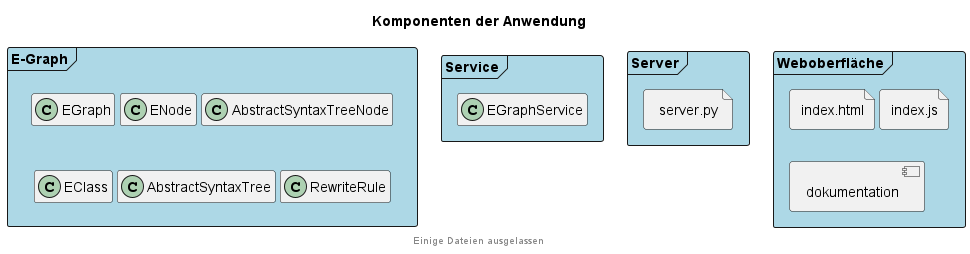
\includegraphics[scale=0.43]{utils/components.png}
        \caption{Architekturdiagramm der Anwendung}
        \label{fig:comps}
    \end{figure}
\end{frame}

\begin{frame}{Ablauf (1)}
    \begin{figure}[H]
        \centering
        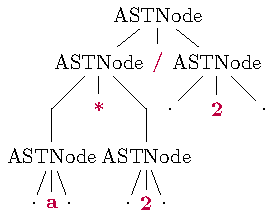
\includegraphics[scale=1.4]{utils/ast.pdf}
        \caption{Abstract Syntax Tree des Ausdrucks $(a \cdot 2) / 2$}
        \label{fig:komponenten}
    \end{figure}
\end{frame}

\begin{frame}{Ablauf (2)}
    
\end{frame}

\begin{frame}{Ablauf (3)}
    
\end{frame}